\documentclass[10pt, a4paper]{report}

\title{Cycling simulation\\or\\\textit{When} to break-away?}
\date{\today}
\author{Dan Demeter\and Robert Kruszewski\and Alexandru P\u{a}unoiu \and C\'esar Prout\'e \and Julian Sutherland}


%\setlength\parindent{0pt}
\usepackage{tabularx, alltt, amsmath, multirow, graphicx, url, graphics}
\usepackage[]{caption}

%Our Executive Summary
\renewcommand{\abstractname}{Executive Summary}

% Better looking chapters headings
\usepackage{titlesec}
\titleformat{\chapter}
  {\normalfont\LARGE\bfseries}{\thechapter}{1em}{}
\titlespacing*{\chapter}{0pt}{3.5ex plus 1ex minus .2ex}{2.3ex plus .2ex}


\begin{document}

\begin{titlepage}

\newcommand{\HRule}{\rule{\linewidth}{0.5mm}} % Defines a new command for the horizontal lines, change thickness here

\center % Center everything on the page

%----------------------------------------------------------------------------------------
%	HEADING SECTIONS
%----------------------------------------------------------------------------------------

\textsc{\LARGE Imperial College London}\\[1.5cm] % Name of your university/college
\textsc{\Large Department of Computing}\\[0.5cm] % Major heading such as course name
\textsc{\large}\\[0.5cm] % Minor heading such as course title

%----------------------------------------------------------------------------------------
%	TITLE SECTION
%----------------------------------------------------------------------------------------

\HRule \\[0.4cm]
{ \huge \bfseries Cycling simulation\\or\\\vspace{0.4cm}\textit{When} to break-away?}\\[0.4cm] % Title of your document
\HRule \\[1.5cm]

%----------------------------------------------------------------------------------------
%	AUTHOR SECTION
%----------------------------------------------------------------------------------------

\begin{minipage}{0.4\textwidth}
\begin{flushleft} \large
\emph{Authors:}\\
Dan Demeter \\
Robert Kruszewski\\
Alexandru P\u{a}unoiu\\
C\'esar Prout\'e\\
Julian Sutherland
\end{flushleft}
\end{minipage}
~
\begin{minipage}{0.4\textwidth}
\begin{flushright} \large
\emph{Supervisor:} \\
Dr. Panos \textsc{Parpas} \\% Supervisor's Name
%Michael \textsc{Hadjiyiannis}
\end{flushright}
\end{minipage}\\[5cm]

% If you don't want a supervisor, uncomment the two lines below and remove the section above
%\Large \emph{Author:}\\
%John \textsc{Smith}\\[3cm] % Your name

%----------------------------------------------------------------------------------------
%	DATE SECTION
%----------------------------------------------------------------------------------------

{\large \today}\\[3cm] % Date, change the \today to a set date if you want to be precise

%----------------------------------------------------------------------------------------
%	LOGO SECTION
%----------------------------------------------------------------------------------------

%\includegraphics{Logo}\\[1cm] % Include a department/university logo - this will require the graphicx package

%----------------------------------------------------------------------------------------

\vfill % Fill the rest of the page with white space
\end{titlepage}

%% Ending of title page

\tableofcontents

\begin{abstract}
During our Group Project we were challenged with analysing cycling races, in particular trying to provide the theoretical foundations for predicting their outcomes. Cycling is amongst the most popular sports worldwide. Its history dates back to the $18^{th}$ century when it was adopted. Since then the number of different types of races has substantially increased: from Track cycling on banks and velodromes to professional races such as the Tour de France. Despite their large popularity and the considerable financing attracted by large races, there is no formal manner of estimating the outcome of a race, not to mention choosing the optimal strategy. In order to achieve the best results choosing the right strategy is essential. Cycling races are extremely exhausting for the organism and timing one's effort carefuly is of paramount importance for winning. One example might be Andy Schleck's victory, during one of the 2011 Tour de France's stage races. His escape 60 km before finish line had been perceived as unimportant by other racers, however, it granted him almost 4 minutes lead at the finish.\\\\
Our work resulted in two tools that can assist one when analysing cycling races. The first of them is an agent based software model, inspired by work done in \cite{AgentModel}, \cite{MathModel} and \cite{SlipStream}, which aims to approximate real races and allows for the simulation of arbitrary scenarios. It makes certain simplyfying assumptions in the physical, psychological and biological models. Because of this, the model is limited with respect to accuracy. Although limited, it has been developed with modularity and the possibility of extension in mind. Even though the agent based model is quite versatile it does not allow strategies to be extracted from it. Hence, alongside the aforementioned model we have also derived a simple game theoretical framework which can be used not only to predict results but also compute optimal strategy for racers. Deriving the game theoretical model from real life scenarios is not an easy task, as shown by \cite{GameTheoryApplications} and \cite{GameTheoryNonTechnical}. The model would be of more use when one would want to make on the spot decisions regarding his strategy.\\\\
In the simulation, we make use of probabilities and randomness to generate more diverse races. On other hand, the game theoretical model does not heavily rely on a probabilistic space. In this paper we analyse the situation of two players breaking away from a group of cyclists and try to generalize this to N players breaking away. We take into account the case when the players can be eventually caught by the chasing group and the one where they are not. Each situation will have an in-depth analysis of the strategies available to players and a discussion of which of them should be applied at a certain moment. Finally, we present a method which should be used to find the optimal strategy. \\\\
In this research project, we aim to present new results and further develop previous work found in the above mentioned papers. We hope these will be of great use in cycling.
\end{abstract}


\chapter{Introduction}\label{ch:intro}

The first cycling race is thought to have been held on the $31^{th}$ of May 1868 in Paris. Nowadays, after roughly 145 years, cycling is one of the top 10 most popular sports during the Summer Olympics \cite{TopEndSportsUrl} and attracts millions of fans worldwide. Cycling competitions are divided into three main categories: \textit{road, track and off-road events}. Like in any popular sport, researcher have shown their interest in methods that could simulate the outcome of races. Efforts have been made to characterize as accurately as possible cycling races. This has led to formulas taking into consideration almost all of the factors that could affect the outcome of the race. Some examples can be seen in \cite{AgentModel} or \cite{SlipStream} .
\\\\
During our project, we have focused mainly on \textit{road events}: \textbf{road race, criterium, hill climbing and stage races} and Sprint \textit{track events}. For a novice watching those competitions, it might seem peculiar the way athletes compete with each other. Even though they are racing against each other, their only chance of success is teaming up with their competitors. Unfortunately, as more members join break-away groups, the rider's chances of crossing the finish line first decreases. However, this can help racers who lack pace as they have the chance to cooperate with others. This behaviour is mostly noted in the Stage Races like the Tour de France or the Tour de Faso in Africa where entire teams that have no chance of winning team up with top teams in order to help them out. Also, during a competition riders can be taken by surprise by their break-away companions who start sprinting towards the finishing line earlier than expected.
\\\\
In the following report we will focus on races where players are forced to cooperate and ask ourselves whether we can derive a game theoretical model that can predict the optimal behaviour for a cyclist. The aims of this project are to first create a cycling race simulation that could realistically reproduce the progress of a race. Secondly, to create a game theoretical framework able to determine the optimal strategy for a cyclist in a certain situation. The final goal is to make it possible to join these together and develop the game theoretical model using data collected from the simulation, as well as include strategies designed from the game theory framework in the simulation.
\\\\
We have managed to create a road race simulation and aimed to make it as realistic as possible. The reader should however take note of the fact that we made certain assumptions. The simulation is described in section \ref{sec:softmodel}. We have also proposed a game theoretical model that  covers the possible outcomes of a race in several types of situations. These where described in section \ref{sec:gameth}. Lastly, we are using the model in order to validate the results from the simulation.

\chapter{Design and Implementation}\label{ch:design&impl}

As can be seen from the introduction, we have split the project into two parts: one is concerned with creating a mathematical model which will be the foundation  for the simulation and the other focuses on game theory and what strategies are best to follow.

\section{The Software Model}\label{sec:softmodel}

In this first part of the project the goal was to be able to describe the setting of a race as accurately as possible: in terms of physical properties (resistance of the wind, friction, etc..) and in terms of physiological and psychological properties of the individuals. Another goal is to be able to determine the outcome of a race run in aforementioned conditions. For that we first considered reproducing the model described in \cite{AgentModel}. It seemed like a fairly easy task at first, but we ran into several complications.

\subsection{The First Model}\label{subsec:model1}

Section 2 of \cite{AgentModel} describes an agent based model for cycling races. Each individual cyclist is represented by its physical and strategic attributes. The cyclists are themselves grouped into packs, any two cyclists that are within three meters of each others are in the same pack. To keep the model manageable, simplifications of the real world had to be made (physical as well as behavioural). In spite of those simplifications, the model still captures the principal elements of professional cycling. \\\\
The goal of packs is to use the slipstream effect cooperatively, taking turns in breaking the wind. Therefore in a pack cyclists rotate to the position of leader (which is more physically demanding), ideally each cyclist in the pack spend the same amount of time being the leader.\\\\
The strategies are defined probabilistically, each cyclist depends on two probabilities to make his decisions. These are distributed normally with mean 0.48 and distribution 0.21 with truncation at 0 and 1. The fist of these probability is the probability of the cyclist acting cooperatively towards his pack, i.e. whether or not he will breakaway and if he is the leader whether or not he will do his share in full. The second one is the probability of acting cooperatively towards your team, i.e. if one of his team mate breaks-away, will he follow him. \\\\
During the race, the cyclists can therefore be in two different states, they are either part of a pack, or breaking away. When they are breaking away, they will stay in a breakaway state for three minutes before forming a new pack or joining an existing one.
\\\\
In the last 5 kilometres of the race, the packs dissolves and each cyclists acts individually and starts sprinting. \\\\
The issue with this model however was with the description of how the cyclists get tired. It was unclear in the paper exactly how it was done, and there was no way of cumulating the energy used. We therefore looked at the description of a better exhaustion and performance model in another paper.

\subsection{The Updated Model}\label{subsec:updmodel}

We used the description of the physical model provided in \cite{MathModel} to update our previous simulation. It has a more precise description of the physical abilities of a cyclist, the motion being based on power output instead of speed, and of the effects of exhaustion. These are described bellow.

\subsubsection{Derivation of the differential equation for modeling the motion of a cyclist}

For the following equations we will use the next symbols: \\

\begin{tabularx}{\linewidth}{|c|X|}
\hline
P is power	&	\_pot is potential energy	\\
T is torque	&	\_air is air drag			\\
F is Force 	&  	\_bear is friction in the wheel bearings \\
			& 	\_roll is the rolling friction (with the road) \\
			& 	\_kin is kinetic energy \\
			&	\_ped is cyclist's 'input' (e.g. $P_{ped}$ = power input into the system) \\
\hline
\end{tabularx}

\begin{tabularx}{\linewidth}{|X|}

$l_{c}$  is the length of the cycling crank \\
% maybe use a parbox here? http://tex.stackexchange.com/questions/485/how-to-break-a-line-in-a-table
$r_{w}$  is the radius of the wheel \\
$\eta$ 		represents the frictional losses in the drive chain \\
$\omega$ 	represents angular velocity.\\
$\gamma$	is the step-up coefficient of the bicycle gearing system.  \\
\hline
\end{tabularx}
\\\\
So by conservation of energy:

$$P_{pot} + P_{air} + P_{bear} + P_{roll} + P_{kin} = \eta * P_{ped}$$
As $Power = Torque * \omega$ , by dividing with $\omega$ we get

$$ T_{pot} + T_{air} + T_{bear} + T_{roll} + T_{kin} = \frac{ \eta * T_{ped} }{ \gamma }  = \frac{\eta * P_{ped}}{\omega * \gamma} $$
From the above notations have $T_{ped}$ = $F_{ped} * l_{c}$ (due to mechanical advantage) and $T = \frac{F * l_{c}}{r_{w}}$ for all the other forces (as there is a dual mechanical advantage between the crank and the wheel).\\\\
This gives us: $$ F_{pot} + F_{air} + F_{bear} + F_{roll} + F_{kin}
	= \frac{ \eta * l_{c} * T_{ped} }{ \gamma }
	= \frac{ \eta * l_{c} * P_{ped} }{ r_{w} * (\omega * \gamma)} $$
As we assume the race is on a perfectly flat surface, then $F_{pot} = 0$. We also assume that the bicycle is 'perfect', so $F_{bear} = 0$. \\\\
This simplifies to: $$F_{air} + F_{kin} = \frac{l_{c} * P_{ped} }{ \omega * \gamma } $$
where $$ F_{air} 	= \frac{1}{2} * c_{d} * \rho * A * ( x'(t) )^{2} $$
and	  $$ F_{kin} 	= ( m + ( \frac{l_w}{r_w^{2}} ) * x''(t) $$
You can also reproduce the above formulas based on research published in \cite{MathModel}.\\\\
We are using the following estimates:
\begin{alltt}
mass of cyclist (m) 				= 63
frontal area of cyclist (A) 		= 0.75
length of crank (\(l_{c}\)) 		= 0.2
air density (\(\rho\)) 				= 1.225 (sea level, 15 degree Celsius)
drag coefficient of a cyclist (d) 	= 0.7
wheel inertia (\(I_w\)) = 0 (as perfect bicycle)
radius of wheel (\(r_w\)) = 0.35
step-up coefficient of gearing (\(\gamma\)) = 7.5
angular velocity of wheels (\(\omega\)) = \(2 * \pi * speed / {r_{w}} \)
\end{alltt}
Therefore the differential equation simplifies to:
$$ 0.3215625 * (x'(t))^{2} + 63 * x''(t)
	= \frac{\eta * l_{c} * P_{ped}} {2 * \pi * x'(t) * \gamma }
	= \frac {0.2 * P_{ped}} {15 * \pi} $$
Which gives approximation of:
$$ 75.7664 *(x'(t))^{3} + 14844.025288499999 * x'(t) * x''(t) = P_{ped}$$
which is a second order non-linear differential equation.\\\\
However this differential equation does not take into account the ``slipstream'' effect.

\subsubsection{Integrating the slipstream effect into the differential equation for modeling the motion of a cyclist.}

The slipstream effect is the effect by which the drag on an object moving through a fluid is diminished by the fact that the fluid it is moving through is already moving at a certain speed due to it being in the wake of another object in motion. \\\\
This can be modelled for cyclists by applying a correction factor ($CF_{draft}$) to $P_{air}$ (which creates the same change in $F_{air}$) in the derivation of the differential equation that depends on the distance between a cyclist and the cyclist in front of him ($d_w$). \\\\\
If $d_w \ge 3$, then $C_{draft} = 1$ as the slipstream effect makes no difference over greater distances (the fluid in the wake of the object in front has the time to stop moving). \\\\
If $d_w < 3$, then $C_{draft} = 0.62 - 0.0104*d_w + 0.0452*d_w^2$ . $^{\cite{SlipStream}}$ \\\\
As in this figure:
\begin{figure}[!ht]
  \centering
    % GNUPLOT: LaTeX picture with Postscript
\begingroup
  \makeatletter
  \providecommand\color[2][]{%
    \GenericError{(gnuplot) \space\space\space\@spaces}{%
      Package color not loaded in conjunction with
      terminal option `colourtext'%
    }{See the gnuplot documentation for explanation.%
    }{Either use 'blacktext' in gnuplot or load the package
      color.sty in LaTeX.}%
    \renewcommand\color[2][]{}%
  }%
  \providecommand\includegraphics[2][]{%
    \GenericError{(gnuplot) \space\space\space\@spaces}{%
      Package graphicx or graphics not loaded%
    }{See the gnuplot documentation for explanation.%
    }{The gnuplot epslatex terminal needs graphicx.sty or graphics.sty.}%
    \renewcommand\includegraphics[2][]{}%
  }%
  \providecommand\rotatebox[2]{#2}%
  \@ifundefined{ifGPcolor}{%
    \newif\ifGPcolor
    \GPcolorfalse
  }{}%
  \@ifundefined{ifGPblacktext}{%
    \newif\ifGPblacktext
    \GPblacktexttrue
  }{}%
  % define a \g@addto@macro without @ in the name:
  \let\gplgaddtomacro\g@addto@macro
  % define empty templates for all commands taking text:
  \gdef\gplbacktext{}%
  \gdef\gplfronttext{}%
  \makeatother
  \ifGPblacktext
    % no textcolor at all
    \def\colorrgb#1{}%
    \def\colorgray#1{}%
  \else
    % gray or color?
    \ifGPcolor
      \def\colorrgb#1{\color[rgb]{#1}}%
      \def\colorgray#1{\color[gray]{#1}}%
      \expandafter\def\csname LTw\endcsname{\color{white}}%
      \expandafter\def\csname LTb\endcsname{\color{black}}%
      \expandafter\def\csname LTa\endcsname{\color{black}}%
      \expandafter\def\csname LT0\endcsname{\color[rgb]{1,0,0}}%
      \expandafter\def\csname LT1\endcsname{\color[rgb]{0,1,0}}%
      \expandafter\def\csname LT2\endcsname{\color[rgb]{0,0,1}}%
      \expandafter\def\csname LT3\endcsname{\color[rgb]{1,0,1}}%
      \expandafter\def\csname LT4\endcsname{\color[rgb]{0,1,1}}%
      \expandafter\def\csname LT5\endcsname{\color[rgb]{1,1,0}}%
      \expandafter\def\csname LT6\endcsname{\color[rgb]{0,0,0}}%
      \expandafter\def\csname LT7\endcsname{\color[rgb]{1,0.3,0}}%
      \expandafter\def\csname LT8\endcsname{\color[rgb]{0.5,0.5,0.5}}%
    \else
      % gray
      \def\colorrgb#1{\color{black}}%
      \def\colorgray#1{\color[gray]{#1}}%
      \expandafter\def\csname LTw\endcsname{\color{white}}%
      \expandafter\def\csname LTb\endcsname{\color{black}}%
      \expandafter\def\csname LTa\endcsname{\color{black}}%
      \expandafter\def\csname LT0\endcsname{\color{black}}%
      \expandafter\def\csname LT1\endcsname{\color{black}}%
      \expandafter\def\csname LT2\endcsname{\color{black}}%
      \expandafter\def\csname LT3\endcsname{\color{black}}%
      \expandafter\def\csname LT4\endcsname{\color{black}}%
      \expandafter\def\csname LT5\endcsname{\color{black}}%
      \expandafter\def\csname LT6\endcsname{\color{black}}%
      \expandafter\def\csname LT7\endcsname{\color{black}}%
      \expandafter\def\csname LT8\endcsname{\color{black}}%
    \fi
  \fi
  \setlength{\unitlength}{0.0500bp}%
  \begin{picture}(7200.00,5040.00)%
    \gplgaddtomacro\gplbacktext{%
      \csname LTb\endcsname%
      \put(1078,704){\makebox(0,0)[r]{\strut{} 0.6}}%
      \put(1078,1163){\makebox(0,0)[r]{\strut{} 0.65}}%
      \put(1078,1623){\makebox(0,0)[r]{\strut{} 0.7}}%
      \put(1078,2082){\makebox(0,0)[r]{\strut{} 0.75}}%
      \put(1078,2542){\makebox(0,0)[r]{\strut{} 0.8}}%
      \put(1078,3001){\makebox(0,0)[r]{\strut{} 0.85}}%
      \put(1078,3460){\makebox(0,0)[r]{\strut{} 0.9}}%
      \put(1078,3920){\makebox(0,0)[r]{\strut{} 0.95}}%
      \put(1078,4379){\makebox(0,0)[r]{\strut{} 1}}%
      \put(1210,484){\makebox(0,0){\strut{} 0}}%
      \put(2142,484){\makebox(0,0){\strut{} 0.5}}%
      \put(3074,484){\makebox(0,0){\strut{} 1}}%
      \put(4007,484){\makebox(0,0){\strut{} 1.5}}%
      \put(4939,484){\makebox(0,0){\strut{} 2}}%
      \put(5871,484){\makebox(0,0){\strut{} 2.5}}%
      \put(6803,484){\makebox(0,0){\strut{} 3}}%
      \put(176,2541){\rotatebox{-270}{\makebox(0,0){\strut{}$CF_{draft}$}}}%
      \put(4006,154){\makebox(0,0){\strut{}$d_w$}}%
      \put(4006,4709){\makebox(0,0){\strut{}Slipstream correction factor ($CF_{draft}$)}}%
    }%
    \gplgaddtomacro\gplfronttext{%
      \csname LTb\endcsname%
      \put(5816,4206){\makebox(0,0)[r]{\strut{}$0.62 - 0.0104*d_w + 0.0452*d_w^2$}}%
    }%
    \gplbacktext
    \put(0,0){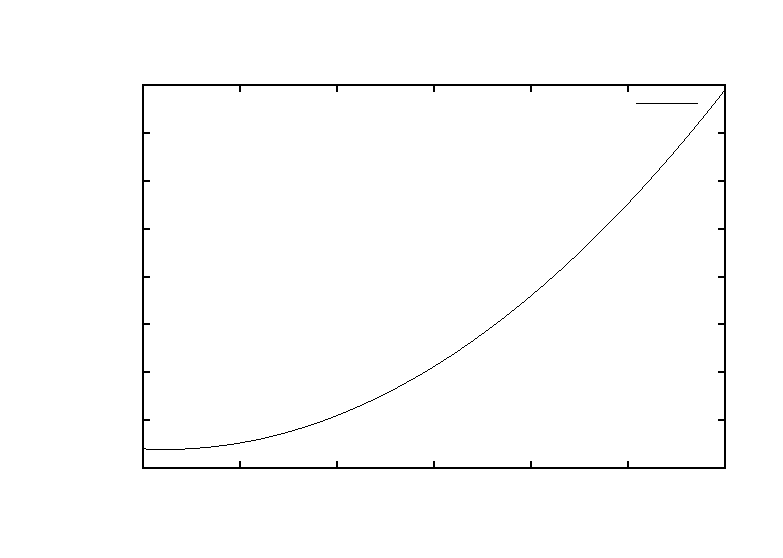
\includegraphics{plot}}%
    \gplfronttext
  \end{picture}%
\endgroup

  \caption{plot of $CF_{draft}$ against $d_w$}
\end{figure}
\\
Note that $CF_{draft} \approx 1$ at $d_w = 3$ on this graph. \\\\
Multiplying $F_{draft}$ by this correction factor gives the new differential equation:
$$ (0.62 - 0.0104*d_w + 0.0452*d_w^2) * 75.7664 *(x'(t))^{3} + 14844.025288499999 * x'(t) * x''(t) = P_{ped}$$
A second order differential equation that models our systems and takes into account the slipstream effect.

\subsubsection{An exhaustion model for cycling}

We add three new constants (all normally distributed) and one new variable to the definition of each cyclist to implement this model. The new constants are :
\begin{itemize}
\item $P_{max}$ : the maximum power output of a cyclist.
\item $P_{CP}$ : the maximum aerobic power output of a cyclist. (The highest speed at which the can cycle without ever getting tired)
\item $E_{an}$ : the maximum energy output from the cyclist anaerobic system before it must rest.
\end{itemize}
The new variable is $e_{an}$ : the amount of the anaerobic energy capacity that has already been consumed (initially $e_{an} = 0$). \\\\
The differential of $e_{an}$ depends on the difference between the cyclist maximum aerobic power output ($P_{CP}$) and his current power output ($P_{ped}$, set according to the psychological model), giving :
$$ e_{an}' = P_{ped} - P_{CP} $$
The values of $e_{an}$ are truncated such that $0 < e_{an} < E_{an}$.

\subsection{The Implementation}\label{subsec:impl}

We decided to implement the above model in Haskell as it allows for highly polymorphic modular code. This allowed us to make the code highly extensible. For example each cyclist can have an independent strategy that can be easily be added to the code. It takes some 'reasonable' amount of information about the surroundings of the cyclist and returns a decision inside the IO Monad allowing for arbitrary side effecting computations to occur. This could allow us to potentially extend it to perform user interaction. \\\\
We split our implementation into these primary modules:
\begin{itemize}
\item \texttt{Cyclist}
\item \texttt{Pack}
\item \texttt{Simulation}
\item \texttt{Modeling}
\item \texttt{RungeKutta}
\item \texttt{Parser}
\item \texttt{Main}
\end{itemize}
We will describe the implementation module by module

\subsubsection{Cyclist}

This module contains the definition the type \texttt{Cyclist}, which represent a individual cyclist, and functions to edit the properties of a cyclists and to generate a certain number of cyclists with particular initial state. \\\\
The type cyclist contains the following variables :

\begin{itemize}
\item \texttt{uid :: Int} \\ A unique id for the cyclist (constant).
\item \texttt{pmax :: Double} \\ The maximum power output (constant).
\item \texttt{pcp :: Double} \\ The maximum anaerobic power output (constant).
\item \texttt{usedEnergy :: Double} \\ Used anaerobic energy, correspond to $e_{an}$ above.
\item \texttt{energyLim :: Double} \\ Maximum anaerobic energy, correspond to $E_{an}$ above (constant).
\item \texttt{packCoop :: RandT StdGen IO Bool} \\ The general cooperation decision function.
\item \texttt{teamCoop :: RandT StdGen IO Bool} \\ The team cooperation decision function.
\item \texttt{groupProb :: Double} and \texttt{teamProb :: Double} \\ If the default cooperation function is used, these stores the probabilities.
\item \texttt{speed :: Speed} \\ Current speed.
\item \texttt{distance :: Meters} \\ Current distance.
\item \texttt{team :: Int} \\ Team number (constant).
\end{itemize}
The types \texttt{Speed} and \texttt{Meters} are defined in \texttt{Units.hs} just to make the code clearer and are synonyms of \texttt{Double}.

\subsubsection{Pack}
The type \texttt{Pack} is defined here. It has two different constructor :

\begin{itemize}
\item \texttt{Pack Int Cyclist (Seq Cyclist) Int} \\ Which correspond to a normal pack. The parameters are respectively : The type the leader spent in this position, the cyclist that is leading, a sequence of the other cyclists in the Pack and an unique pack id.
\item \texttt{Breakaway (Seq Cyclist) Int Int} \\ Which correspond to a breakaway pack. The parameters are respectively : The sequence of cyclists in the pack, the number of turns before the pack becomes a normal pack, and an unique pack id.
\end{itemize}
The module also contains the functions \texttt{defLeader} and \texttt{rotate} which are used to enforce the rotation of the cyclist in the leading position. The \texttt{defLeader} function will start a rotation if the current leader has been in this position for five turns or if he decides to act as a defector and not finish his share. \\\\
The rest of the module is composed of utility functions to facilitate the use of packs.

\subsubsection{Simulation}
This is the core of the software. It defines the type \texttt{Race} like this :
\begin{itemize}
\item \texttt{Race Int Meters [Pack] [Cyclist] [(Cyclist, Double)]} \\ where the parameters are : the current turn number, the total length of the race, a list of the packs in the main part of the race, a list of the cyclists that are in the sprinting phase in the last five kilometres of the race, and a list of the cyclists that have finished the race, coupled with their finish time.
\end{itemize}
The principal function is \texttt{turn} which is called repeatedly to go from one state of the race to the next one. The algorithm it performs is as follows :

\begin{enumerate}
\item Generate the new breakaway packs. We go through every cyclist in each pack and call their strategy function to know if they will breakaway, or if a team-mate breaks-away, if they follow him and form the new breakaway packs.
\item Update the leaders of each pack if needed, by calling \texttt{defLeader} of the \texttt{Pack} module on each of them.
\item Update the speed of the riders, which is defined in the \texttt{Modelling} and \texttt{RungeKutta} modules that describe the physical model.
\item Update their position from their speed. Here we also check for collisions between packs, in which case the colliding packs are merged into one.
\item Update their energy, from their current energy and $P_{ped}$ in \texttt{Modelling}.
\end{enumerate}

\subsubsection{Modelling}

The Modelling module of this simulation contains all the function necessary to update the speed and pack structure of a cyclist either in the normal part of the race (breakaway group or pack) and that for updating the speeds of the sprinters. \\\\
For cyclists that are in a breakaway group or in a pack, we compute the average power of the cyclists in the grouping and set their speed to 80\% or 90\% of the speed achievable at this power output. For sprinters, the speed is set to that possible with 95\% of their \texttt{pmax}. This module calls the \texttt{RungeKutta} module below for computing the speed of each cyclist depending on his power output and his previous speed.

\subsubsection{RungeKutta}

% Initial equations
To model the we have of the motion of cyclists requires us to solve the differential equation:

$$ 75.7664 *(x'(t))^{3} + 14844.025288499999 * x'(t) * x''(t) = P_{ped}$$
for x'(t), the speed of the cyclist. \\\\
Unfortunately, this is a non-linear differential equation, which in general has no analytic equation (i.e. in general, no equation can be found in terms of the variables in the equation which gives a solution to $x'$).\\\\
So we decided to use a numerical solving algorithm to solve for x'(t) so we could compute the change in velocity of our cyclists over time.\\\\
Runge-Kutta is a standard numerical method that allows one to estimate a function based on an initial value and the function's differential. It is similar to the standard ``newton method" ($f(x + h) \approx f(x) + h*f'(x)$), but it uses several points inside a trapezium to trace the function significantly better. \\\\
This allows approximations to be made for functions for which we have a first order differential equation. It can also be used to approximate $n$ interdependent functions if it has an initial value for each and a differential that depends on the $n - 1$ other functions' values at $x$ and on $x$ itself.\\\\
So as above we have the differentials of $n$ functions denoted $y_1'(t),..,y_n'(t)$, which can each be written as: 
$$y_k'(t) = f_k(t,y_1(t),y_2(t),..,y_{(k-1)}(t),y_{(k+1)},..,y_n(t))$$
The each of the differentials can be given the current value of t and the $n - 1$ previous estimated values (initially the initial values) of the other function and then running Runge-Kutta with respect to t on each of them with a small h. \\\\
This means that if we can transform our second order differential equation into a system of two first order coupled differential equations from which the information we want can be analytically derived, we can use the Runge-Kutta method to solve it numerically and then derive any necessary values from the result. \\\\
In order to apply the Runge-Kutta algorithm, we need to transform it into two linear differential equations. We will define 2 independent variables, $y_1$ and $y_2$ such that their differentials $y_1'$ and $y_2'$ must depend on the variables t, $y_1$ and $y_2$. Let
$$ y_1' = f( t, y_1, y_2 )$$ and $$y_2' = g( t, y_1, y_2 )$$
In order to get x'(t) we want to set one of the equations to contain it: $y_1 = x'(t)$ and because we want one of the equations to contain $x'(t) * x''(t) $ so set: $y_2' = x'( t ) * x''( t )$ .
This gives us $$ y_{2} = \frac{1}{2} * x'(t)^2 $$
By rearranging the differential equation to have only $ x'( t ) * x''( t )$ on the left hand side, we get
$$ x'( t ) * x''( t ) = \frac{P_{ped} - 75.7665 * x'( t ) ^ 3}{14844.025288499999}$$
$$ y_2' = \frac{P_{ped} - 75.7665 * y_1 ^ 3}{14844.025288499999}$$
Now we have only $y_2'$ in terms of only t, $y_1$ and $y_2$ so we can set $$ g( t, y_1, y_2 ) = \frac{P_{ped} - 75.7665 * y_1 ^ 3}{14844.025288499999}$$
Writing $y_1$ in terms of t, $y_1$ and $y_2$: $$y_2 = \frac{1}{2} * x'(t)^2$$ yields $$y_2 = \frac{1}{2} * y_1^2$$
And by rearranging the left hand side we get:
$$y_1 = \sqrt{2 * y_2}$$
Now we differentiate with respect to $t$:
\begin{align*}
y_1' & = \frac{y_2'}{\sqrt{2 * y_2}}\\
& = \frac{P_{ped} - 75.7665 * y_1 ^ 3}{14844.025288499999 * \sqrt{2 * y_2}}
\end{align*}
This gives us the final form for function f:
$$ f(t, y_1, y_2) = \frac{P_{ped} - 75.7665 * y_1 ^ 3}{14844.025288499999 * \sqrt{2 * y_2}}$$
To take the slipstream effect into account, we only have to make a relatively small modification (only the movement to the left hand side changes for $y_2'$ changes, adding a dependence on $d_w$):
$$ f(t, y_1, y_2) = \frac{P_{ped} - 75.7665 * (0.62 - 0.0104*d_w + 0.0452*d_w^2) * y_1 ^ 3}{14844.025288499999 * \sqrt{2 * y_2}}$$
$$ g( t, y_1, y_2 ) = \frac{P_{ped} - 75.7665 * (0.62 - 0.0104*d_w + 0.0452*d_w^2) * y_1 ^ 3}{14844.025288499999}$$
$d_w$ can either be set to the initial value at the beginning of the minute or changed dynamically, but this requires a simultaneous simulation of all the cyclists to see how they change in real time, which is quite complex.\\\\
The solution of these coupled differential equations via the Runge-Kutta algorithm is implemented in the RungeKutta module using Haskell 'prim-ops', to make it extremely fast.

\subsubsection{Parser}

This module is used to parse an input file to generate a race. The syntax of the input file is as follows:
\begin{itemize}
\item The first line contains only one number: the length of the race.

\item Each of the following lines contains the description of one type of cyclist, and the number of that type of cyclist you want to assign to a number of teams.
\begin{itemize}
\item We first write a list of \texttt{team\_number:number\_of\_cyclists}
\item then a $|$ to act as separator
\item the name of the strategy function, possibly followed by arguments between brackets. (e.g. standardCoop takes a distribution as argument)
\item another $|$
\item a list of \texttt{property:value} to define the properties of the cyclist, \texttt{property} must be one of the variable of the \texttt{Cyclist} type, except for the strategy variables. If a property is omitted, a default value is assigned.
\end{itemize}
An example of such a line could be : \\ \texttt{1:20 5:10 | standardCoop avg | pcp:1.28}
\end{itemize}
The module works by parsing a \texttt{String} then calling the generating functions of the \texttt{Cyclist} module and creates a \texttt{Race} with the generated cyclists.

\subsubsection{Main}

The \texttt{Main} module of this program contains the \texttt{main} function.
The main function parses the arguments to the program and loads any required input file.\\\\
The arguments that can be passed to the program are:
\begin{itemize}
\item ``-X'': Activates the graphical interface that shows an accelerated rendering of the race.
\item ``-P'': Outputs a plot that is defined in the code (This could be extended to having a configurable plotting feature).
\end{itemize}
The main function then loads the input file and generates the corresponding race by using the parser. It then calls turn repeatedly until the Race has finished, giving a graphical representation if the ``-X'' option is given. It then outputs the results of the race and a plot if the ``-P'' option is given.

% Game theoretical model introduction

\section{Game Theory Model}\label{sec:gameth}

In order to create a thorough mathematical model we aim to construct a game theoretical model. This model will help racers to change their strategies and choose the optimal one as the race unfolds. To create a sound model, we based our assumptions on the simulation previously described. We managed to abstract the mathematical foundations of the simulation to develop the game theory.\\\\
Modelling bike races can be quite challenging, hence we will begin with the simplest case in order to introduce our methodology and explain the simplifying assumptions we are making. When participating in a race we can argue that racers are at each point faced with three possible options: either break-away from their current group or fall back to the group preceding the current one or cooperate with the other members of the group (which essentially implies copying the strategy of the other players in their group - which will be discussed later). Each of the racers can change his mind as often as he wants, however, changes in strategy will likely incur penalties on their performance. In this section we try to determine whether there is a dominant strategy and try to find at which point in race it is beneficial for racer to change his strategy. We can easily see that strategy chosen by players will depend on their skills and fitness, i.e. better racers can afford more aggressive, less cooperative strategy in hope of being able to outdistance opponents. On the other hand weaker players will tend to cooperate more. The difficulty of this part is not the actual solution to the model since it might happen there will not be a general solution but fitting the model to the actual situation. It is fairly easy to construct arbitrary theoretical games, however, when the games have to even remotely represent reality they get complicated very quickly.\\\\
Before we can dive into discussion of game theoretical models we have created we aim to present short introduction to game theoretical concepts we are using. Also short a summary of core principles of game theory is included with references to further readings. We then continue to consideration of cases with two racers when the group chasing them is very far from them and does not affect the strategies. Thus, they are guaranteed to come first and second.

\subsection{Definitions}\label{subsec:defs}

Before we can indulge ourselves in discussion of game theory can be used to approach bicycle racing problem we must introduce the terms we are making use of.

\paragraph{2-person Zero-sum Game} ~\\
Two-person zero-sum game describes conflict of interest between two players with strictly opposite interests. Formally this means that any change in the pay-off of one player has to be offset with equal decrease in amount of payout to the second player. These types of games can be divided into three subsections depending on the achievable results to the game. We can have a dominant strategy equilibrium, pure strategy Nash equilibrium and mixed strategy Nash equilibrium each with less strictness imposed on the result.
\paragraph{Dominant Strategy Equilibrium}
is represented by the table below. Ease of analysing such games stems from the fact that there is always a clear strategy that a player has to follow in order to achieve maximum payout.\\

% Dominant strategy equilibrium derivation %

\begin{table}[ht!]
	\hspace{-4em}
	\centering
	\begin{tabular}{ccccc|}
		& & \multicolumn{3}{c}{Player 1}                                \\ \cline{3-5}
		& & A & B & \multicolumn{1}{c}{C}                               \\ \cline{3-5}
		\multirow{3}{*}{Player 2} & \multicolumn{1}{|c|}{a} & 2 & 1 & 7 \\
		& \multicolumn{1}{|c|}{b} & 4 & 5 & 6                           \\
		& \multicolumn{1}{|c|}{c} & 3 & 1 & 7                           \\ \cline{3-5}
	\end{tabular}
	\caption{2-person zero-sum game\\ dominant strategy equilibrium}
\end{table}
\noindent In order to find a dominant strategy equilibrium we need to find a dominant strategy.
\paragraph{Row player} strategy $i$ dominates strategy $j$ (for row player) if $\forall k. a_{ik} \ge a_{jk}$ and $\exists k.a_{ik} > a_{jk}$.
\paragraph{Column player} strategy $i$ dominates strategy $j$ if $\forall k. a_{ki} \le a_{kj}$ and $\exists k.a_{ki} < a_{kj}$.
\\\\
Using these rules we can reduce the pay-off matrix. It is clear that strategy $C$ is dominated by either $A$ and $B$. Hence, the matrix is reduced to:
\begin{table}[ht!]
	\hspace{-4em}
	\centering
	\begin{tabular}{cccc|}
		& & \multicolumn{2}{c}{Player 1}                            \\ \cline{3-4}
		& & A & \multicolumn{1}{c}{B}                               \\ \cline{3-4}
		\multirow{3}{*}{Player 2} & \multicolumn{1}{|c|}{a} & 2 & 1 \\
		& \multicolumn{1}{|c|}{b} & 4 & 5                           \\
		& \multicolumn{1}{|c|}{c} & 3 & 1                           \\ \cline{3-4}
	\end{tabular}
	\caption{2-person zero-sum game\\ dominant strategy equilibrium}
\end{table}
\\\\
Furthermore one can spot that both strategies $a$ and $c$ are dominated by $b$
\begin{table}[ht!]
	\hspace{-4em}
	\centering
	\begin{tabular}{cccc|}
		& & \multicolumn{2}{c}{Player 1}           \\ \cline{3-4}
		& & A & \multicolumn{1}{c}{B}              \\ \cline{3-4}
		Player 2 & \multicolumn{1}{|c|}{b} & 4 & 5 \\ \cline{3-4}
	\end{tabular}
	\caption{2-person zero-sum game\\ dominant strategy equilibrium}
\end{table}
\\\\
Which comes down to the following :
\begin{table}[ht!]
	\hspace{-4em}
	\centering
	\begin{tabular}{ccc|}
		& & \multicolumn{1}{c}{Player 1}       \\ \cline{3-3}
		& & \multicolumn{1}{c}{A}              \\ \cline{3-3}
		Player 2 & \multicolumn{1}{|c|}{b} & 4 \\ \cline{3-3}
	\end{tabular}
	\caption{2-person zero-sum game\\ dominant strategy equilibrium}
\end{table}
\\
Hence the final and dominant strategy pair is $(A,b)$.

% Pure Nash equilibrium derivation

\paragraph{Pure Nash Strategy Equilibrium} represents a situation when no player has an incentive to deviate from the strategy chosen, since no player can choose a better strategy given the choices of the other players. Consider the following table.
\begin{table}[ht!]
	\hspace{-4em}
	\centering
	\begin{tabular}{ccccc|}
		& & \multicolumn{3}{c}{Player 1}                                  \\ \cline{3-5}
		& & A & B & \multicolumn{1}{c}{C}                                 \\ \cline{3-5}
		\multirow{3}{*}{Player 2} & \multicolumn{1}{|c|}{a} & 11 & -7 & 8 \\
		& \multicolumn{1}{|c|}{b} & 1 & 1 & 2                             \\
		& \multicolumn{1}{|c|}{c} & -10 & -7 & 21                         \\ \cline{3-5}
	\end{tabular}
	\caption{2-person zero-sum game\\ pure strategy Nash equilibrium}
\end{table}
\\
To put Nash strategy equilibria in simpler words the row player (Player 2) wants to maximise minimal gain from the game and column player (Player 1) wants to minimise maximal payout of the game. We can then easily derive Nash strategy equilibrium by looking at rows and following the rules. Consider the table below.
\begin{table}[ht!]
	\hspace{-4em}
	\centering
	\begin{tabular}{ccccc|c}
		& & \multicolumn{3}{c}{Player 1} &                                     \\ \cline{3-5}
		& & A & B & \multicolumn{1}{c}{C} & min                                \\ \cline{3-5}
		\multirow{3}{*}{Player 2} & \multicolumn{1}{|c|}{a} & 11 & -7 & 8 & -7 \\
		& \multicolumn{1}{|c|}{b} & 1 & 1 & 2 & 1                              \\
		& \multicolumn{1}{|c|}{c} & -10 & -7 & 21 & -10                        \\ \cline{3-5}
		& max & 11 & 1 & \multicolumn{1}{c}{21} &
	\end{tabular}
	\caption{2-person zero-sum game\\ pure strategy Nash equilibrium}
\end{table}
\\
The resulting table allows to easily point the Nash equilibrium. Another way of looking at this solution is to realise that it is a saddle point in the graph of strategy space. Hence, neither of the players has incentive to deviate from it. In case of above matrix one can deduce that Nash equilibrium is at $(B,b)$.

\paragraph{Mixed Strategy Nash Equilibrium} is a situation when there is no pure strategy, hence we cannot state that one strategy is always better than the other. However, we can still obtain a solution to this game by assigning probabilities to strategies. By playing strategies according to their corresponding probabilities one can achieve optimal expected output of the game. Following table show situation like this
\begin{table}[ht!]
	\hspace{-2em}
	\centering
	\begin{tabular}{cccc|c}
		& & \multicolumn{2}{c}{Player 1} &                                \\ \cline{3-4}
		& & A & \multicolumn{1}{c}{B} & min                               \\ \cline{3-4}
		\multirow{2}{*}{Player 2} & \multicolumn{1}{|c|}{a} & -1 & 5 & -1 \\
		& \multicolumn{1}{|c|}{b} & 3 & -5 & -5                           \\ \cline{3-4}
		& max & -3 & \multicolumn{1}{c}{5} &
	\end{tabular}
	\caption{2-person zero-sum game\\mixed strategy Nash equilibrium}
\end{table}
\\
There is no pure equilibrium strategy, however, on can be found using Linear Programming techniques. If we apply such technique to this problem we will find out the following probabilities (given in brackets) for this game.
\begin{table}[ht!]
	\hspace{-2em}
	\centering
	\begin{tabular}{cccc|}
		& & \multicolumn{2}{c}{Player 1}                                               \\ \cline{3-4}
		& & A \textit{(0.7143)}& \multicolumn{1}{c}{B \textit{(0.2857)}}               \\ \cline{3-4}
		\multirow{2}{*}{Player 2} & \multicolumn{1}{|c|}{a \textit{(0.5714)}} & -1 & 5 \\
		& \multicolumn{1}{|c|}{b \textit{(0.4286)}} & 3 & -5                           \\ \cline{3-4}
	\end{tabular}
	\caption{2-person zero-sum game\\mixed strategy Nash equilibrium}
\end{table}

\paragraph{2-person Non-Zero-sum Game} ~\\
Non-zero-sum game turn out to be considerably more difficult to analyse properly. Even though we are usually able to find optimal strategy it might not be the best strategy. Furthermore when game is played more than once, strategy presumed to be optimal in single case might not be the most effective one. The most famous example of such game is the Prisoner's Dilemma. Albert W. Tucker formalised this problem giving it its name:
\begin{quotation}
\textit{
    Two members of a criminal gang are arrested and imprisoned. Each prisoner is in solitary confinement with no means of speaking to or exchanging messages with the other. The police admit they don't have enough evidence to convict the pair on the principal charge. They plan to sentence both to a year in prison on a lesser charge. Simultaneously, the police offer each prisoner a Faustian bargain. If he testifies against his partner, he will go free while the partner will get three years in prison on the main charge. Oh, yes, there is a catch ... If both prisoners testify against each other, both will be sentenced to two years in jail.}
    \end{quotation}
Above description can be represented by pay-off matrix like this:
\begin{table}[ht!]
	\hspace{-2em}
	\centering
	\begin{tabular}{cccc|}
		& & \multicolumn{2}{c}{Player 2}                                              \\ \cline{3-4}
		& & Stay Silent &  \multicolumn{1}{c}{Testify}                                \\ \cline{3-4}
		\multirow{2}{*}{Player 1} & \multicolumn{1}{|c|}{Stay Silent} & (1,1) & (3,0) \\
		& \multicolumn{1}{|c|}{Testify} & (0,3) & (2,2)                               \\ \cline{3-4}
	\end{tabular}
	\caption{Prisoner's Dilemma pay-off matrix}
\end{table}
\\
We will leave it to the reader to find optimal strategy for this game as it turns out to be quite rewarding task. One can also consider whether his or hers strategy will change if the game is to be played more than once.

\paragraph{N-person Game} ~\\
Considering N-person games leaves much to be desired from. One of the problems is that possible strategies can grow exponentially with number of players, hence, these problems are at least more computationally difficult than 2-person games. Also when a player is faced with more than one equivalent, however, differing in terms of pay-off option will not always choose the strategy guaranteeing highest pay-off. Furthermore interpersonal factors come into play and are of great significance and players need to carefully consider what inducements they must offer and accept. In our work we do not consider pure N-person games, however, we present how with respect to cycling races such cases can be simplified with some level of accuracy.
\\\\
For deeper and more detailed explanation the reader is encouraged to make himself familiar with contents of \cite{GameTheoryNonTechnical} or \cite{GameTheoryApplications}. Further in the work we assume that reader is at least familiar with the concepts presented above.

\paragraph{Breaking away} ~\\
We assume that when a cyclist breaks-away he does so with maximum possible speed. Hence, he is expending as much energy as possible.

\paragraph{Cooperation} ~\\
For a racer to cooperate means to follow the strategy of the racers in the group. If there are more than two racers we assume that the racers willing to cooperate will cooperate with breakaways and not stay in the group. When there are no breakaways cooperation we will preserve the current status of the game.

\paragraph{Fall back} ~\\
When a racer falls back he limits his velocity so that he will get caught by the group preceding the one he is part of at the moment of making the decision. If there is no group to fall back to the racer moves to a further position in the group. This action isn't instantaneous, however we assume that racers will not form a group between falling back from one group to another.

\paragraph{Value Of A Game} ~\\
For a zero-sum game the value of that game is the expected value to one of the players when both play a perfect strategy.

\paragraph{One-off Game} ~\\
This is a game played at some moment $\delta^{(n)}$ before race finish line which determines payoff at given moment.

\subsection{2-racer Escape Case}\label{subsec:zerosumgame}
Let us consider the length of the race to be $R > 0$. In order to reason about the pay-off of each player when choosing a certain strategy during the race, it is best to single out a moment when the choice of each player is clear. Hence, in the case we are currently discussing (two racers broke away from the chasing group and it is certain they cannot be caught), we easily realize that in the last $\delta\ km$, where $\delta\ll R$, the two players will definitely choose to breakaway and push as hard as possible in order to win the race. This will have pay off $C_i>0$ for player $i$, where $i \in \{1,2\}$.
\\\\
Let us now consider the moment $\delta'$, with $\delta'>\delta$ and $\delta'\ll R$. We can easily infer that the pay off for each player $i$ is $\max\{C_i,V_{\delta'_i}\}$, where $V_{\delta'_i}$ is the value of the one-off game at moment $\delta'$ for player $i$. By continuing in this manner we get that at moment $\delta^{(n)}$, with $\delta^{(j)}>\delta^{(i)}$ for all $j>i$ and $\delta^{(0)}=\delta$ we have that the pay off for each player $i$ is $P_{i,n} = \max\{P_{i,n-1},V_{\delta^{(n)}_i}\}$, where $P_{i,0} = C_i$. Hence, we have deduced a recursive relation that lets us easily reason about the choice of strategies.
\\\\
In order to get the one-off game pay-off matrices we need the following formulas:\\
$CS_{i,n} = \dfrac{P_{ped_{i,n}} \cdot \delta^{(n)}}{E_{i,n} \cdot x},\ i\in\{1,2\}$ - the interpretation of this coefficient is the proportion of energy we have to reach finish at given speed, calculated at moment $\delta^{(n)}$. It is specifying in terms of current pedalling power of the cyclist $P_{ped_{i,n}}$, the remaining energy $E_{i,n}$ and his current speed $x$.\\\\
$F_{draft}(x)=(0.62 - 0.0104d_w + 0.0452 d_w^2)\cdot (1/2)\cdot c_d\cdot \rho\cdot A\cdot x^2$ -  represents the force applied to the cyclist due to the aerodynamic drag from the air taking into account the slipstream effect. In this case the $x$ is the speed of the cyclist. We remind the reader that $d_w$ is the distance between the two cyclists.
$P = \dfrac{CS_{1,n}}{CS_{1,n}+CS_{2,n}}$ - the probability of player 1 being in front on player 2 at moment $\delta^{(n)}$ depending on their $CS_{i,n}$.
\\\\
We will list the possible strategy combinations with their respective pay-off players might use during the game. Before doing so, let us define $F_{max}$ to be the maximum draft a player can attain, and $F_{min}$ the minimum one.
\\\\
\textbf{Player 1 Cooperates, Player 2 Cooperates}
\\
The pay-off for Player 1 is $(1-P)\cdot F_{draft}(s_1)$ and $P \cdot F_{draft}(s_2)$ for Player 2, where $s_i$ is the speed of Player $i$. The pay-off for the two players is as such because if they cooperate they gain an advantage by drafting one behind the other ($F_{draft}(s_i)$). This advantage, however, is greater for the player behind as he will put less effort, hence we need the probability $P$ of Player 1 having first place.
\\\\
We now need to normalize these quantities such that we get a pay-off in the interval [1,2], where 1 represents the worst pay-off (i.e. second place) and 1 the best (i.e. first place). After normalization we get that the pay-off for Player 1 is $(1-P)\cdot \dfrac{F_{draft}(s_1)}{F_{max}} + 1$ and the one for Player 2 is $P\cdot \dfrac{F_{draft}(s_2)}{F_{max}} + 1$.
\\\\
The reasoning behind the normalization is as follows:\\
Let us consider the pay-off for Player 1 (for Player 2 the reasoning is similar). Notice that if $P=1$, then the formula is 0. Let us multiply it by a normalization coefficient $N$ and add 1 to the formula. We get $(1-P)\cdot N\cdot F_{draft}(s_1)  + 1$. Thus, if we replace $F_{draft}(s_1)$ by $F_{max}$, then this yields the following inequality: $(1-P)\cdot F_{max} \cdot N + 1\le 2$. After several easy computations we get $N = \dfrac{1}{F_{max}}$. Replacing it in the equation, we get the result. Note that the other inequality - $\ge 1$ - holds trivially.
\\\\
\textbf{Player 1 Cooperates, Player 2 Breaks-away}
\\
Player 1's pay-off is clearly the same as before, i.e. $(1-P)\cdot \dfrac{F_{draft}(s_1)}{F_{max}} + 1$ - after normalization. Because of the fact that Player 2 breaks-away then his pay-off depends on his positioning i.e. $1-P$, but we must also take into account whether or not he is trailing behind Player 1 and hence, if he can get any benefit from drafting. Thus, we have two disjoint probability events and we can argue that the pay-off is $(1-P) +  P\cdot \dfrac{F_{draft}(s_2)}{F_{max}} + 1$ - after normalization. To explain it a bit more, $P\cdot \dfrac{F_{draft}(s_2)}{F_{max}}$ this is the part of the pay-off that tells him the benefit he gets from drafting. We then want to specify that his pay-off also depends on the probability of him being in front and hence we add $1-P$. It is to remark the fact that we are still in the [1,2] interval as the events (trailing or leading) are disjoint.
\\\\
\textbf{Player 1 Cooperates, Player 2 Falls back}
\\
\textit{Note.} In this case by falling back, the reader should understand that Player 2 wants to trail behind Player 1 such that he can benefit from drafting. We have this interpretation because there is no chasing group that should be taken into account and thus, this is the only rational choice he can make.
\\\\
By the note above we conclude that the pay-off for the two players are $(1-P) +  P\cdot \dfrac{F_{draft}(s_1)}{F_{max}} + 1$ and $(1-P)\cdot \dfrac{F_{draft}(s_2)}{F_{max}} + 1$ for Player 1 and Player 2 respectively. Notice that the pay-offs are similar as in the situation above, only that they are swapped.
\\\\
\textbf{Player 1 Breaks-away, Player 2 Cooperates}
\\
Similar pay-off as in the case \textit{Player 1 Cooperates, Player 2 Breaks-away}. Only the order changes.
\\\\
\textbf{Player 1 Breaks-away, Player 2 Breaks-away}
\\
In this case both players stop cooperating and they depend solely on their performance which is computed by $P$ and $1-P$. Thus, we can argue that the pay-off for Player 1 is $P+1$ and the one for Player 2 is $2-P$, after normalization.
\\\\
\textbf{Player 1 Breaks-away, Player 2 Falls back}
\\
This is an interesting case, because Player 2 might play 'sneaky' and try to fall back and then benefit from drafting by chasing the player that broke away. However, we won't treat this situation because we want to preserve simplicity and because this case implies that Player 1 doesn't really manage to break-away. Thus, we conclude that the pay-off in this case is $P+1$ for Player 1 and 1 for Player 2.
\\\\
\textbf{Player 1 Falls back, Player 2 Cooperates}
\\
Similar pay-off as in the case \textit{Player 1 Cooperates, Player 2 Falls back}. Only the order changes.
\\\\
\textbf{Player 1 Falls back, Player 2 Breaks-away}
\\
Similar pay-off as in the case \textit{Player 1 Breaks-away, Player 2 Falls back}. Only the order changes.
\\\\
\textbf{Player 1 Falls back, Player 2 Falls back}
\\
In this case, we set both pay-offs to 1 (worst pay-off) because this strategy does not fully apply to our case.
\\\\
Now, we can trivially build a pay-off matrix containing the values we deduced above.\\\\
Pay-off of the game theoretical model resembles the rules outlined in \cite{AgentModel} after which our simulation has been created. We identified independent variables and made them influence pay-off values since this way we can generalise it to all types of players. Also it gives us basis for comparison which results will be shown later.\\\\
\textit{Note.} The reader may notice that we didn't specify the distance $d_w$. This should be varied in the simulation such that we can see which distance between the players is the optimal one for choosing certain strategies.

\subsection{Getting Caught}\label{subsec:getcaught}
Everything seems fairly simple when there are only two racers competing. Entering realm of n-player games leaves us with few definite results as more interpersonal qualities come into play. It is an important to know that communication, players attitude towards each other and perceived strength of a player in a game can influence strategies chosen. However, we separate on case where we can get some results.
\\\\
For a case when two racers have escaped and are being chased by peloton we can consider scenarios when there exists a possibility of them being caught. It is no longer a zero-sum game since players can drop below $2^{nd}$ place and one can lose without other gain. However, we are not considering the chasing peloton as players. We are merely treating them as moving group of people that has a potential of catching up with the escape group.
\\\\
First we need to quantify the chance of being caught. Actually since we can know the distances between racers, their velocity and we can measure the time it is not only a possibility, but certainty. This holds as long as one of the groups does not change its strategy when we have to re-evaluate the chance. Consider $\epsilon \in \{0,1\}$, it has value of 0 if the escape group consisting of our players will not be caught and 1 otherwise. We set $\epsilon$ at moment $\delta^{(n)}$ to 1 if $\frac{x}{v_{draft}}=\frac{x+d}{v_{group}}$ has a solution in range $0\le x\le d$ where $d$ is the distance from the peloton to the escape group, $v_{draft}$ and $v_{group}$ are the velocities of the second (drafting) racer in escape and the peloton (chasing group) respectively. Knowing value of $\epsilon$ we can simplify our model to considering two cases: one when players will safely reach finish first and secondly when they will be absorbed by the peloton. It is easy to notice that the first case has been mostly solved in the previous section, it only needs few adjustments. Also it is not difficult to derive pay-offs for the absorbed case since players are likely to get places depending on their fitness across whole race group (it clearly would not be the case if all racers were considered to be players and were allowed to choose strategies as racers will react differently when chasing tired racers from escape).
\\\\
When trying to deduce the pay-off matrix one can notice that this problem can be divided into two cases - depending on the value of $\epsilon$ - which will finally yield in two matrices. These matrices will be swapped during the game depending on the situation players face.
\\\\
\textbf{$\epsilon$ is zero}
\\
This case is one that it is easily dealt with considering the work we need in the previous section. By having $\epsilon = 0$, it means that we could ignore the group from the equation and the matrix pay-off is, hence, identical to the one we got before.
\\\\
\textbf{$\epsilon$ is one}
\\
This case is a bit more interesting, but it can be easily solved by adding some extra observations on top of the previous game theoretical model. Before doing so, we define some more formulas that will be used.\\
$CS_{race} = \sum\limits_{i=1}^{N} CS_i$, where $N$ is the number of players in the game. \\
The first observation is that in some cases normalization will take place on the interval $[1,N]$. This is because the two front-runners can become part of the pack.\\
The relevant situations are those when one of the two players decides to fall back - this time to the chasing group - or wants to break-away. We decided that the rest of the situations should be treated as in the case above, maybe with normalization on $[1,N]$ instead of $[1,2]$.\\\\
Thus, when one of the players falls back, then his pay-off becomes $\dfrac{CS_i}{CS_{race}}$ where $i\in\{1,2\}$. Of course now we need to normalize this quantity on $[1,N]$. As we are on the interval $[0,1]$, the immediate solution is multiplying by $N-1$ and adding 1. The pay-off we get is $ \dfrac{CS_i}{CS_{race}}\cdot (N-1) + 1$. The next question is, what will the other player do? If the strategy is fall back as well, then his pay-off is calculated in a similar manner. Otherwise, any strategy will have the pay-off of the break-away strategy described in the previous model.

\subsection{Repeated Game}\label{subsec:repgame}
We can consider our methodology of finding pay-off for the whole game with alteration allowing for change of strategy in order to allow optimal value of the game. Evaluating our model this way enables us to answer questions of optimal strategies at given points in time.\\\\
In order to evaluate the games presented above, we reduced everything to solving 3 by 3 one-off games. After doing this, we plug the values into the recursive formula and we get the required value of the game. Furthermore once we store the pay-off matrices at given $\delta^{(n)}$ moments we can find and optimal strategy trail from beginning to the end. Using search algorithms we could then attempt finding optimal strategies for given scenario. However, such computation would be very computationally intensive since search space grows exponentially with number of moments.

\subsection{N-player Cooperative Game}\label{subsec:nplaycoopgame}
This is the field we have touched least on since Game Theory offers very little with respect to identification methodology of solving this cases. When there are more than 2 players most of the rationality taken for granted in 2 player zero-sum games no longer applies. However, we could try and reduce everything to 2 player games, even though the results might not be as exact. The idea is to average the performance of $N-1$ players in order to create a new player. We will make this new player compete with the $N$th player. Thus, we reduce this to a 2 player game.\\\\
The reader may notice that we need to apply N-player games when the front-runners from the previous sections get caught by the chasing group. Here would be a place where we can apply the aforementioned reasoning. Another idea is to transform this game into an LP problem and solve it using classic algorithms.

\subsection{Solving a 3 x 3 Matrix Game}
In this section we will present an idea (due to \cite{TheoryOfGames}) to solve 3 x 3 matrix games, which can then be easily applied to the pay-off matrices we created before. As described in the next chapter, this will be of an important practical usage provided it will be implemented in the simulation.\\\\
At this moment, we do not know, without having any values as input, which strategies are dominant at a moment in time. Thus, we would like to solve this game in a mixed strategies fashion. Let us try to find the solution for Player 1 and take $X=(x_1,x_2,x_3)$ such that he will choose strategy $i$ with probability $x_i$. Our goal is to find the optimal $X$, denoted by $X^*$. Consider the pay-off matrix to be $A = (a_{ij})$ and let us define its columns as $\bar{a}_j$.\\\\
We can write the following equations:
$$x_1\ge 0,\ x_2\ge 0,\ x_3\ge 0$$
$$x_1+x_2+x_3=1.$$
Hence, in order to find the optimal $X^*$ it is sufficient to look what happens inside the triangle $\triangle$ with vertex coordinates $(1,0,0)$, $(0,1,0)$, $(0,0,1)$. We note that all of the points $X$ are inside $\triangle$ and that the value of our game is $v = \max\limits_{X\in \triangle}\min\limits_{j} X\bar{a}_j$. Now, we make the observation that each $X\bar{a}_j$ defines a line and that each two either intersect or they are parallel (may also coincide). By writing the system of equations $X\bar{a}_j = X\bar{a}_i$ one can remark that we end up splitting the triangle into three regions $R_1$, $R_2$, $R_3$ and we can rewrite our value $v$ as: $$v = \max\limits_{j}\big{\{}\max\limits_{X\in R_j} X\bar{a}_j\big{\}}.$$
For each region we obtain , in order to find the maximum it is sufficient to look at the coordinates of vertices (by the \textit{Fundamental Theorem of Linear Programming}). For more details on this we refer the reader to \cite{TheoryOfGames}.

\chapter{Conclusion And Evaluation}\label{ch:concl}

% What did we manage to do ? \\

% What have we learned ? \\

% What could have been done differently ? \\

% What could we do next ? \\

This project presents a functional simulation of cycling races. It might be a simple one, but it captures the important elements of road cycling. It has been made with modularity in mind, the input format allows to describe easily a wide range of situation in details, and even if only one type of strategy has been implemented, we made sure it would be easy to add more advanced ones. Related to the front-end however, we believe that the project would benefit from a GUI extension, with a better representation of the race. The GUI could have the possibility to analyse the outcome more in depth: being able to generate plots to analyse the effect of different strategies or physical abilities. It could also be created such that you can have the option to pause the race and inspect various parameters and values. We believe that being able to pause a simulation and analyse that specific situation in-depth would be a powerful feature for the GUI.
\\\\
This project could also benefit from a proper documentation. As we mentioned earlier above, we have separated our code into multiple small \textit{modules} in order to make the code more flexible. Unfortunately we don't have a documentation describing the format of the input and how to add extensions to the simulation. This is also due to the various and multiple incremental changes in our modules, as we were adjusting the code.\\\\
A further extension could look into trying to make the simulation and the game theoretical framework work together to produce new results. We could be able to analyse more complex games with information gained from tests on the simulation, for example to determine the pay-off of different strategies. It would also be possible to implement very complex strategies, based on game theory and add them to the simulation. \\\\
By having the game theory model and the simulation working more closely together, we can implement a 3 x 3 matrix game solver (each player has three possible strategies, as mentioned in the previous chapter). See previous chapter for a detailed solution idea. Moreover, a next step is to formalize the idea of the N-person game and try to solve the resulting N-dimensional game. In addition, as the simulation develops further, we can start taking into account, in the game theory model, the altitude the cyclists race at, as this can have an impact on their performance.
\\\\
Overall, it was a great experience working collaboratively on a project with no fixed boundaries, where we had to research and create our objectives. To achieve more  results however, we would have to work on a better time management and organisation. Also, in order to test our Game Theory strategy, we could have run our simulation in a distributed fashion instead of just running it multiple times on our machines. We could have implemented this by using Condor which is already installed on our lab machines.


\chapter{Project Management}\label{ch:projmanag}

\section{Overview}\label{sec:pmoverview}
As our project consisted of two parts very different in nature, we divided the work between two subgroups. Julian Sutherland and C\'{e}sar Prout\'{e} worked on creating the software simulation, and Alexandru P\u{a}unoiu, Dan Demeter and Robert Kruszewski worked on the game theoretical model. We held weekly meetings with our supervisors, to asses the work of the previous week and fix the goals for the next one. We had regular meetings in order to keep everyone updated on the general progress of the work and decide upon the next step of the work.
\\\\
In the simulation team, we worked closely together during the whole duration of the project. We made sure both of us agreed on the design decisions before writing any code. We usually worked together on the same part of the code or divided the work into small individual tasks. However, we still faced difficulties. The biggest one being underspecification of models presented in the source material. Despite our attempts to contact the authors, we didn't manage to find any other pieces of information. Because of this we developed our own alternative model, which is built upon parts of the different papers we read.
\\\\
On the other hand, for the Game Theory initially we started our research individually. After that, we have discussed the methodology with our supervisor and this led to a draft Game Theory model. We believe that the weekly meetings we had where the most important ones, as the feed-back received by the supervisor was very valuable towards getting to the final model. The biggest problem with agile methodologies is that they are specifically designed for writing code and not mathematical models. 
%
%
% All of  the mathematical model team took Operations Research course which in our supervisor mentioned as a prerequisite, however, we have found the content of the course to be lacking with respect to actually setting up the game
%
                                                                                                                                                                                                                                                                                                                                                                     
                                                                                                                                                                                                                                                                                                                                                                     %TODO here All of us needed some time in order to learn the basic Game Theory concepts, which despite being simple, were more in depth than the  ones normally taught during ou lectures. Material available often is concerned with solving imaginary games, where the one closest resembling reality is the prisoner's dilemma. Our problem, however, was entirely different from the one considered by most authors in the field of Game Theory. Our task was to develop model that would give results to real situation. Every game considered by game theory resembles some aspect of reality, however, none of them is dependent on physiology of players, those games only consider mental effort that everyone is capable of. We think that biological conditions of players play great part in computing the results since, you can only go so fast on a bike.
\\\\
Due to the nature of our courses we did not always manage to solve issues when they arrived. Because our different obligations for other modules and work applications made the communication between people working on different parts of the project difficult at times. Due to the non deterministic nature of learning, there have been weeks during which we managed to make significant progress and others that were not very productive. Furthermore, coursework and the fact that three out of five members decided to take more optional modules than average also had an impact on the progress.

\section{Software Engineering Practices}\label{sec:softeng}
Compared to past group projects, what made the biggest difference in the way we had managed this project were software engineering practices - especially agile development. As our project was a mix of mathematical modelling and software development we had initially struggled to adapt these techniques to our needs. What we discovered in the process was that agile development was invented with software development and does not necessarily match well with learning mathematics, especially when the material is completely new and one does not know which parts will become useful later on. We managed to make the system work for us by making incremental changes to our understanding and work, however, these have been difficult to judge. At the point when all of us sufficiently understood background material we did not have problem with adjusting to weakly meetings schedule. Even with these issues, we managed to adapt quickly to the work schedule.
\\\\
The other aspect that was initially problematic was the group size. All of us have never before worked on software engineering project in a group larger than three and from our experience the difference of two members, even tough appears marginal, completely changes projects dynamics. When there is a possibility of two separate streams of development it is of paramount importance to keep everyone updated and resolve issues quickly. Furthermore synchronisation between the two is crucial so that one subgroup will not sit idly. We managed to achieve independence mainly due to the fact that the two parts of the project were separate. Even though we still experienced idle time due to sporadic misunderstanding of our role in project. Again, the software engineering practices were helpful here, as we quickly started  using git as a distributed revision control and source code management. This is why during the Christmas break, when all our team members left London we  successfully managed to collaborate.
\\\\
Throughout the project we learned to greatly appreciate material taught during our courses as it has proven invaluable.

\section{Acknowledgements}\label{sec:ack}
We would like to express our greatest thanks to Dr. Panos Parpas ( our supervisor ) and his PhD student, Michael Hadjiyiannis, without whom we would not have made such progress and the project would have not reached the state it is in currently.

% To add something to the bibliography, look for the "import into BibTex" thingy on google scholar, and add the stuff into refs.bib.
\bibliographystyle{plain}
\bibliography{refs}

\end{document}
